\documentclass[UTF8,zihao = -4]{ctexart}
\usepackage{pdfpages}
\input{data/en_preamble}


%% 首页格式
%\input{data/shouye}

%\numberwithin{table}{section}
%\numberwithin{figure}{section}
%\usepackage[labelsep=quad]{caption}
%\makeatletter
%\def\fnum@figure#1{\figurename\nobreakspace\thefigure\hspace{1em}}%去掉图后面的冒号并加空白空1em
%\def\fnum@table#1{\tablename\nobreakspace\thetable\hspace{1em}}%去掉表后面的冒号并加空白1em
%\makeatother

%%%% 导言区结束
%%%%%%%%------------------------------------------------------------------------

%%%%%%%%------------------------------------------------------------------------

%%%% 公共信息
\jsxm{高星} %教师姓名
\jyszr{高星}	%教研室主任
\jc{《数控机床编程与操作(数控铣床加工中心分册)》沈建峰}%教材
\cks{《加工中心编程与操作》刘加孝主编}%参考书
\skbc{2017级大专数控班}%授课班次
\biaoti{理论}%标题头

%%%% 正文部分
\begin{document}
%\addcontentsline{toc}{section}{封面-前}
%\begin{titlepage}
%	
%\begin{center}
%{ \zihao{1} \bf
%\makebox[10cm][s]{湖南九嶷职业技术学院}  \\
%\makebox[10cm][s]{湖南潇湘技师学院} \\ }
%\vfill 
%{ \zihao{1} \fangsong  \fontsize{46pt}{80pt}\selectfont
%   教\par 案\par 本\par }
%\par
%\vfill \vfill \zihao{4} \setlength{\baselineskip}{1cm}  \bf  
% 授课教师:\underline{ \makebox[5cm]{ \jsxmNR}}\par
% 授课课程:\underline{ \makebox[5cm]{ 数铣编程与操作}}\par
%授课班级:\underline{ \makebox[5cm]{ \skbcNR}} 
%\vfill
%{\bf 二O一八 }——{\bf 二O一九}~~学年\hspace{0.5cm} 第~{\bf 一}~学期
%\end{center}
%\vfill
%
%\end{titlepage}

%\newpage
%\input{data/shoukejihua}
%\restoregeometry
%\newpage

%\tableofcontents
%
%\thispagestyle{empty}
%\addcontentsline{toc}{section}{授课计划}
%\includepdf[pages={-},landscape=true]{16jdzb-skjh.pdf}

\zihao{4}
\setcounter{section}{3}%重新计数
\setcounter{page}{1}
%\include{data/sec1}
%\include{data/sec2}
%\jxhj{%教学后记
	}
\skrq{%授课日期
	2017年9月21日 1-2节}
\ktmq{%课题名称
	基本指令及写程序思路 }
\jxmb{%教学目标,每行前面要加 \item
	\item 掌握手工编程的流程;
    \item 掌握基本指令;
    \item 编写矩形凸台的程序;
    \item 掌握编程基本思路。}
\jxzd{%教学重点,每行前面要加 \item
	\item 掌握G90、G91、G0、G1指令;
	\item 编写数控程序的基本思路;}
\jxnd{%教学难点,每行前面要加 \item
	\item 掌握G90、G91、G0、G1指令;}
\jjff{%教学方法
	通过讲述、举例、演示法来说明;}

\makeshouye %制作教案首页

%%%%教学内容
\subsection{组织教学}
\begin{enumerate}[1、]
	\item 集中学生注意力;
	\item 清查学生人数;
	\item 维持课堂纪律;
\end{enumerate}
\subsection{复习导入及主要内容}
\begin{enumerate}[1、]
    \item 数控编程的坐标系及假设;
    \item 数控程序的结构;
    \item 数控程序的指令;
    \item 数控编程的方式;
    \item 编写程序的基本思路。
\end{enumerate}
\subsection{教学内容及过程}
\subsubsection{案例分析}

在数控铣床或加工中心上加工如图\ref{fig:3-1}所示的零件,试完成程序的编写,已知毛坯为 $\Phi$ 110*30。

\begin{figure}
    \centering
    \includegraphics[width=0.8\linewidth,trim=50 150 50 100,clip]{data/image/3-1.jpg}
    \caption{}
    \label{fig:3-1}
\end{figure}

\begin{enumerate}[1、]
    \item 图样分析;
    \item 确定加工内容;
    \item 确定装夹及工件坐标系;
    \item 确定刀具及切削用量;
    \item 确定工序及走刀路线;
    \item 计算点坐标;
    \item 编写程序单。
\end{enumerate}

\subsubsection{程序名}
1、Fanuc的程序号与Siemens的程序名

Fanuc中用程序号区分各程序,程序号由位址O跟4位数字构成;是号,也就是说O0001号与O1号,表示同一个程序。

注意:1-7999为用户区域

8000-8999为加锁用户区域

9000-9999为厂方提供(扩展功能如O9001为换刀程序,也是加锁的)

所以用户最好别用8000-9999这些号码

2、Siemens中用程序名来区分各程序,确定程序名的规则是:

A、开始的两个符号必须是字母

B、其后的符号可以是字母,数字或下划线

C、最多为16个字符

D、不得使用分隔符

\subsubsection{安全注销指令}
1、G54-G59  选用工件坐标系,(后面讲)。

2、G17-G19  加工平面选择:

G17:XY平面 第一轴为X轴

G18:YZ平面 第一轴为Y轴

G19: ZX平面 第一轴为Z轴

圆弧指令、刀具半径补偿指令、钻孔指令等使用之前有设定平面。

3、G40、G49、G80 取消半径补偿、长度补偿、钻孔循环。

4、G90、G91 绝对坐标编程 增量坐标编程

G90指令按绝对坐标方式设定输入坐标,即移动指令终点的坐标值X、Y、Z都是以工件坐标系统坐标原点(程序零点)为基准来计算。

G91指令按增量坐标方式设定输入坐标,即移动指令终点的坐标值X、Y、Z都是以始点为基准来计算,再根据终点相对于始点的方向判断正负,与坐标轴正方向一致则取正,相反取负。

一般用G90,需要时采用G91,用完应立即改成G90。

\subsubsection{主轴正反转}
M3 S\verb|____| 主轴正转,其中S设定主轴转速,单位为r/min.

注意:本学校的机床,只有加工中心可以用S,数控铣床是机械调速,S无效,Siemens上不能使用S,不然机床会一直等主轴到达设定的转速后,才接着执行后面的程序。

\subsubsection{位移指令G0、G1}
定位(G0)

G00指令使刀具以绝对或相对指令快速移到工件系统指定的位置。在绝对指令状态下,编程端点的坐标值。在相对指令状态下编程中刀具移动的距离。

[ 格式 ]

G00 IP\_\_;

IP\_\_ :
对于绝对指令,端点的坐标值。对于相对指令,是指刀具移动的距离。

[ 说明 ]

刀具轨迹通常不是一条直线。

G00指令的快速移动速度是由参数No.1420由机床制造商来设定的。在实际执行G00时,刀具在单节的开始加速到预先指定的速度并在单节的结束减速。在确认到位后执行下一单节。到位的含义是指进给马达在指定的误差范围内。这个范围是由制造商在参数No.1826中设定的。

刀具沿直线移动。

[ 格式 ]

G01 IP\_\_ F\_\_ ;

IP\_\_ : 对于绝对指令,指端点的坐标,相对指令是指刀具移动的距离。

F\_\_ : 刀具进给的速度(进给率)

[ 说明 ]

刀具以指定的进给率F沿直线移动到指定的位置。

进给率F有效直到赋予新值,不需要在每个单节都指定。

F码指定的进给率是沿刀具轨迹测量的。

如果不指定F值,则认为进给率为零。

每个轴的进给率方向如下:

[ 限制 ]

G01 αα ββ γγ ζζ Ff  ;

α轴方向的进给率:Fα=α/L ×f

β轴方向的进给率:Fβ=β/L ×f

γ轴方向的进给率:Fγ=γ/L ×f

ζ轴方向的进给率:Fζ=ζ/L ×f

L2 = α2 + β2 + γ2 + ζ2

[ 举例 ]

■直线插补


\subsubsection{编写程序的基本思路}
程序初始化(安全保护)--------辅助准备(换刀,主轴启动,切削液开)--------定位到起刀点--------快速下刀--------工进下刀--------走加工轮廓--------提刀---------快速提刀到安全平面-------程序结束(换刀,主轴停止,切削液关,程序返回等)
\subsection{课堂小结}
\begin{enumerate}[1、]
\item 案例分析;
\item 指令讲解;
\item 编写程序;
\item 编写程序的基本思路。
\end{enumerate}
\vfill
\subsection{布置作业}
\begin{enumerate}[1、]
	\item 自定尺寸,编写加工一个矩形外形的程序?
\end{enumerate}
\vfill
\jxhj{%教学后记
	}
\skrq{%授课日期
	2017年9月21日 3-4节}
\ktmq{%课题名称
	基本指令(一) }
\jxmb{%教学目标,每行前面要加 \item
	\item 掌握G1与G0的区别。
    \item 掌握G2/G3的基本应用。
    \item 掌握编写数控程序的基本思路。
    \item 了解数控常见指令。}
\jxzd{%教学重点,每行前面要加 \item
	\item 掌握G1与G0的区别;
	\item 掌握G2/G3的基本应用;}
\jxnd{%教学难点,每行前面要加 \item
	\item 掌握G2/G3的基本应用;}
\jjff{%教学方法
	通过讲述、举例、演示法来说明;}

\makeshouye %制作教案首页

%%%%教学内容
\subsection{组织教学}
\begin{enumerate}[1、]
	\item 集中学生注意力;
	\item 清查学生人数;
	\item 维持课堂纪律;
\end{enumerate}
\subsection{复习导入及主要内容}
\begin{enumerate}[1、]
\item 案例分析;
\item 指令讲解;
\item 编写程序;
\item 编写程序的基本思路。
\end{enumerate}


\textbf{G0与G1的区别}

\begin{enumerate}[1、]
\item 指令格式不同:G1使用前必须用F设定进给速度,G0的速度与F无关 
\item 运动轨迹不同:G0为快速定位,其路径可能为直线,也可能为折线。G1为直线插补,其路径为直线。
\item 进给速度不同:G0的速度由机床参数及快速倍率决定,档位少。G1的速度由F及进给倍率决定,可调档位多。
\item 功能用途不同:G0用于加工前的定位及加工后的提刀,G1用于车削加工
\end{enumerate}
注意:

新学的同学用G1 F2000 代替 G0 (可控与不可控)

不要三坐标编程,定位时,先提刀,再定位。

\subsection{教学内容及过程}
\subsubsection{案例分析}

在数控铣床或加工中心上加工如图\ref{fig:4-1}所示的零件,试完成程序的编写,已知毛坯为 $\Phi$ 110*30。

\begin{figure}[h]
    \centering
    \includegraphics[width=0.8\linewidth,trim=50 150 50 100,clip]{data/image/4-1.jpg}
    \caption{}
    \label{fig:4-1}
\end{figure}

\begin{enumerate}[1、]
    \item 图样分析;
    \item 确定加工内容;
    \item 确定装夹及工件坐标系;
    \item 确定刀具及切削用量;
    \item 确定工序及走刀路线;
    \item 计算点坐标;
    \item 编写程序单。
\end{enumerate}

\subsubsection{G02/G03指令(只讲R编程)}

常见的圆弧标注—— 半径

起点——终点——半径

圆弧插补指令:

1、[格式]
XpYp平面的圆弧   
G17  G2/G3  X\_ Y\_ R\_ F\_
ZpXp平面的圆弧   
G18 G2/G3 Z X R F 
YpZp平面的圆弧   
G19 G2/G3 Y Z R F
对于我们学校的一般用G17平面

指令格式的说明

G17	指定圆弧在XpYp平面

G18	指定圆弧在XpZp平面

G19	指定圆弧在YpZp平面

G02	顺时针方向圆弧插补(CW)

G03	逆时针方向圆弧插补(CCW)

Xp\_\_	X轴或平行于X轴的指令值(由参数No.1022设定)

Yp\_\_	Y轴或平行于Y轴的指令值(由参数No.1022设定)

Zp\_\_	Z轴或平行于Z轴的指令值(由参数No.1022设定)

R\_\_	圆弧半径指定的带符号的圆弧半径

F\_\_	沿圆弧的进给率 



2、圆弧插补的方向

在XpYp平面(ZpXp平面或YpZp平面)“顺时针方向”(G02)和“逆时针方向”(G03)是从笛卡尔坐标系的Zp轴(Yp轴或Xp轴)去看正负方向来决定的,

3、目标点坐标

用位址Xp,Yp,Zp指定的圆弧的端点是根据G90还是G91来表达是绝对值还是相对值。

对于相对值, 终点的距离要从指定圆弧的起点来看。

4、举例:

A-B   G91   G90 

……   ( 学生练习)




\subsubsection{编写程序的基本思路}
程序初始化(安全保护)--------辅助准备(换刀,主轴启动,切削液开)--------定位到起刀点--------快速下刀--------工进下刀--------走加工轮廓--------提刀---------快速提刀到安全平面-------程序结束(换刀,主轴停止,切削液关,程序返回等)
\subsection{课堂小结}
\begin{enumerate}[1、]
\item 案例分析;
\item 指令讲解;
\item 编写程序;
\item 编写程序的基本思路。
\end{enumerate}
\vfill
\subsection{布置作业}
\begin{enumerate}[1、]
	\item 自定尺寸,编写加工一个矩形外形的程序?
\end{enumerate}
\vfill
%\include{data/sec5}
%\include{data/sec6}
%\include{data/sec7}
%\include{data/sec8}
%\include{data/sec9}
%\include{data/sec10}
%\include{data/sec11}
%\include{data/sec12}
%\include{data/sec13}
%\include{data/sec14}
%\include{data/sec15}
%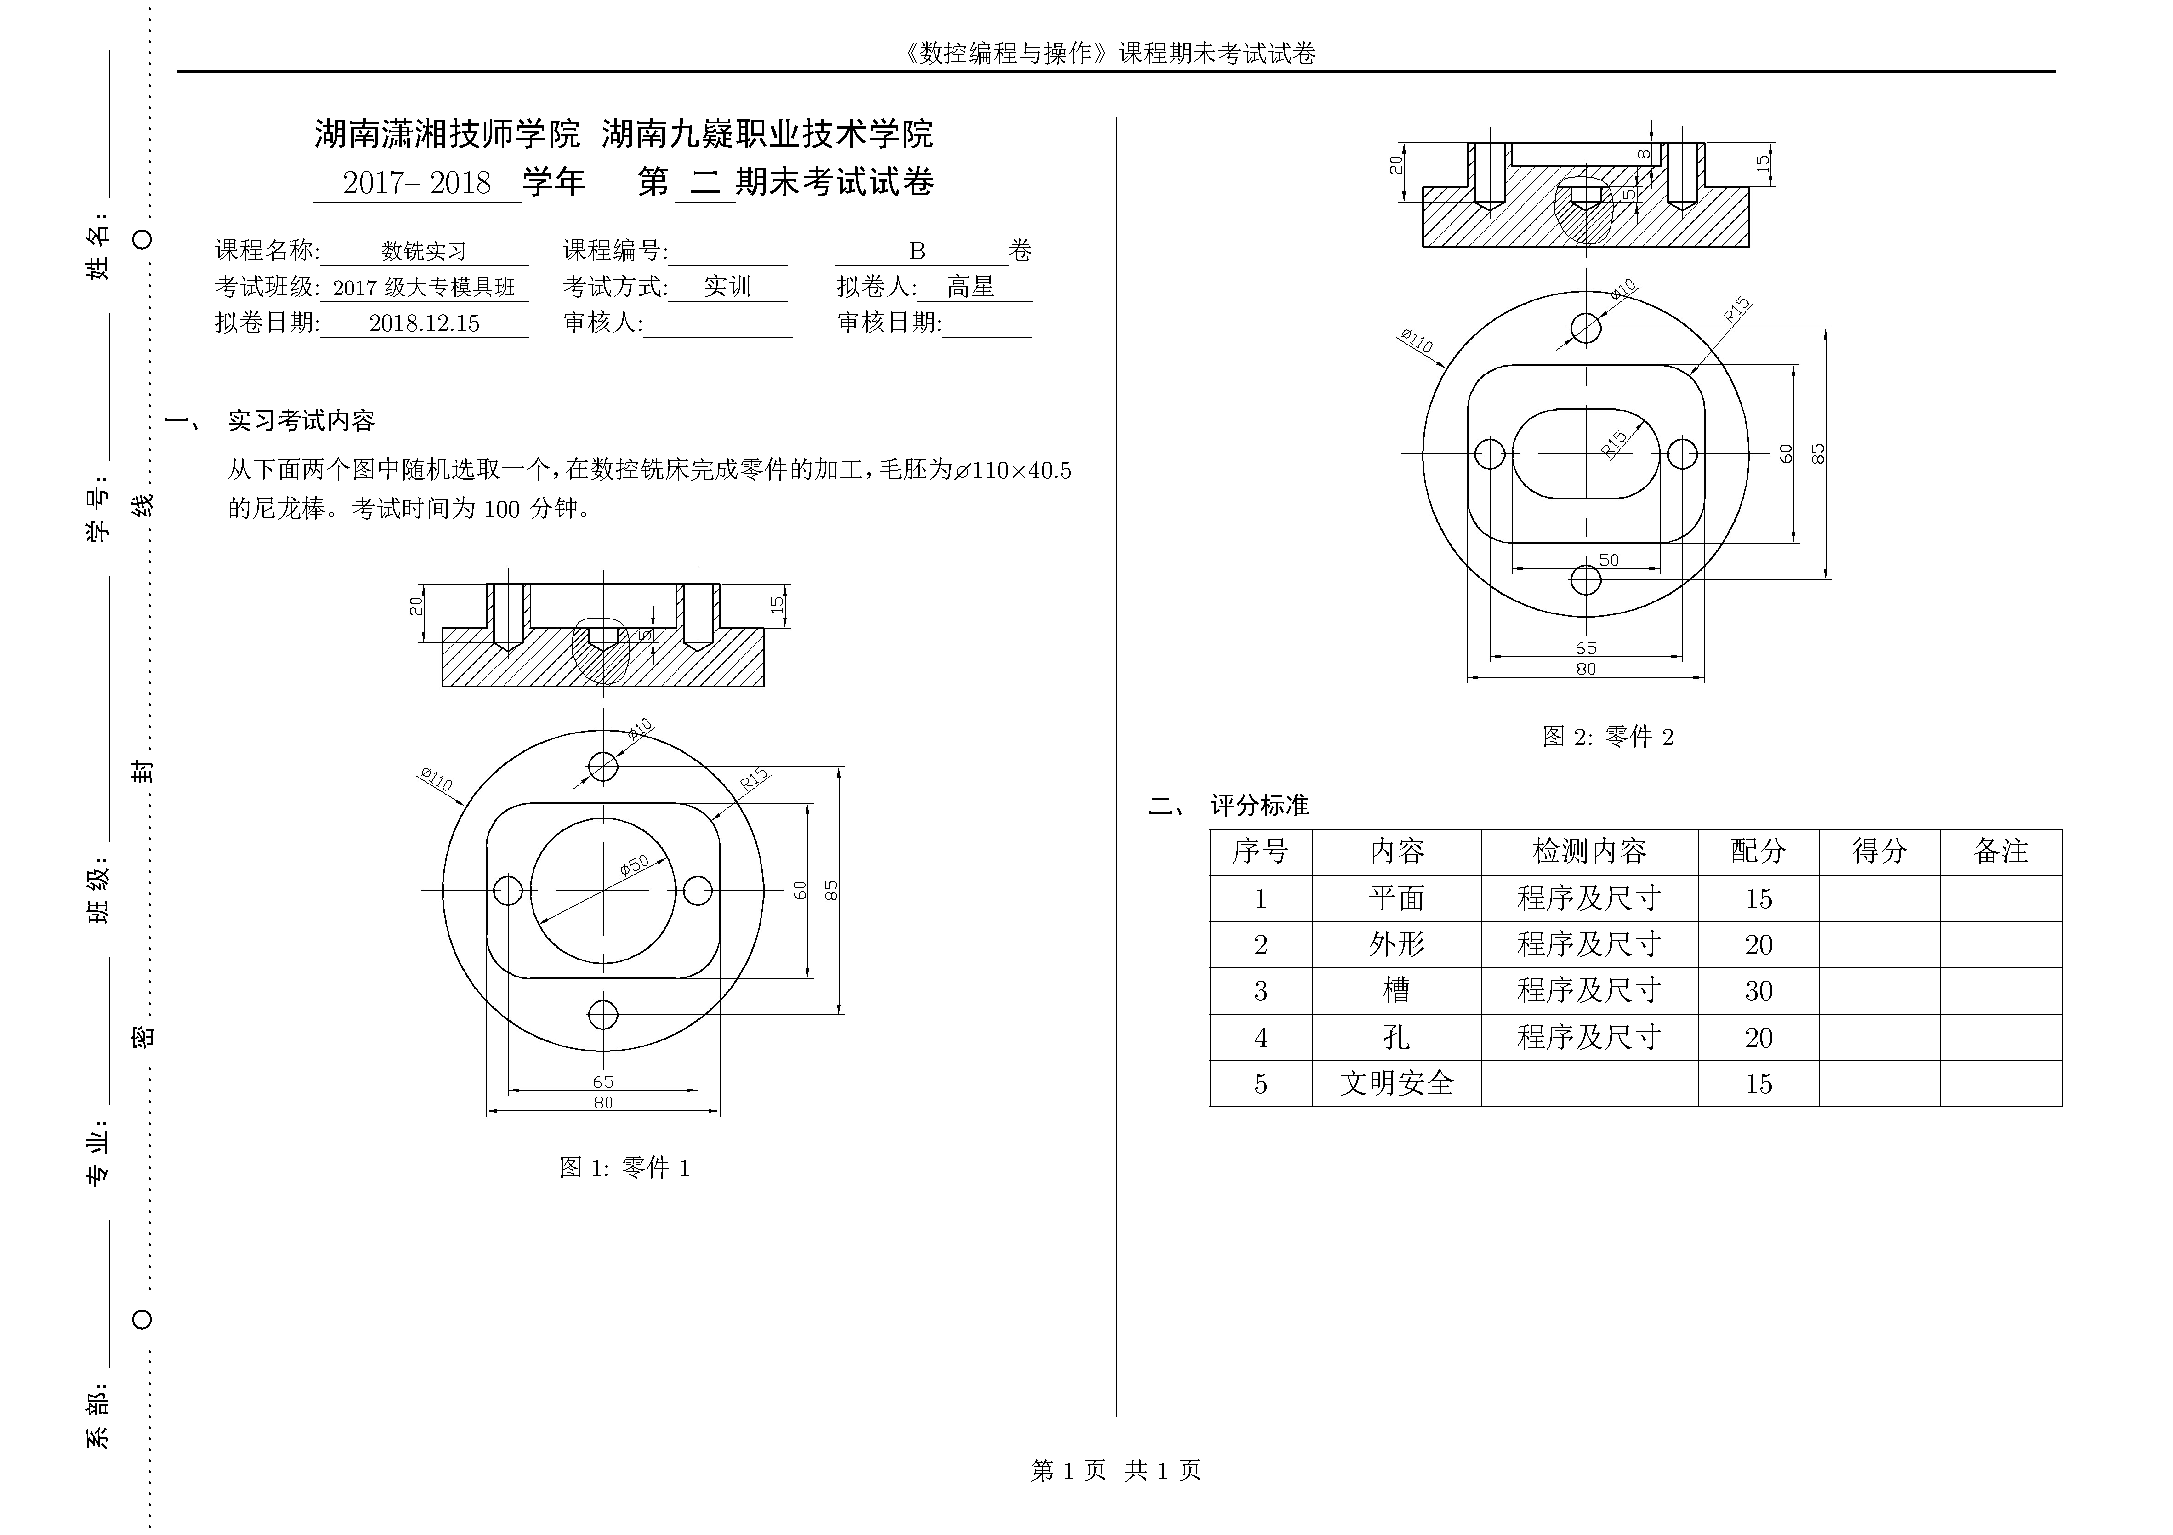
\includepdf[pages={-},landscape=true]{shijuan.pdf}
%\include{data/sec16}
%\includepdf[pages={-},landscape=true]{shijuan-daan.pdf}
%\include{data/sec17}
%\include{data/sec18}
%\include{data/sec19}
%\include{data/sec20}
%\include{data/sec21}
%\include{data/sec22}
%\include{data/sec23}
%\include{data/sec24}
%\include{data/sec25}
%\include{data/sec26}
%\include{data/sec27}
%\include{data/sec28}
%\include{data/sec29}
%\include{data/sec30}
%\include{data/sec31}
%\include{data/sec32}
%\include{data/sec33}
%\include{data/sec34}
%\include{data/sec35}

\biaoti{实习}%标题头
%重新设定目录
%\titlecontents{section}[0pt]{\addvspace{5pt}\filright}
%{ 实习  \thecontentslabel \hspace{0.5em} }
%{}{\titlerule*[8pt]{.} \contentspage}
%\include{data/sec16}

\setcounter{section}{0}%重新计数
\ctexset {
	section = {
		name = {实习},
	}
}

%\include{data/shixi_1}
%\include{data/shixi_2}
%\include{data/shixi_3}
%\include{data/shixi_4}

\newpage
\newgeometry{top=2cm, bottom=2cm, left=2.cm, right=2.cm,includehead,includefoot}
\fancyhead{} 
\chead{ }
\lhead{ } %边框 
\rhead{ }%边框 
\zihao{-4}	
%
%\newpage 
%\newgeometry{top=2cm, bottom=1.5cm, left=2cm, right=2cm,includefoot}
%
%\newpage
%\thispagestyle{empty}
%\addcontentsline{toc}{section}{期末试卷}
%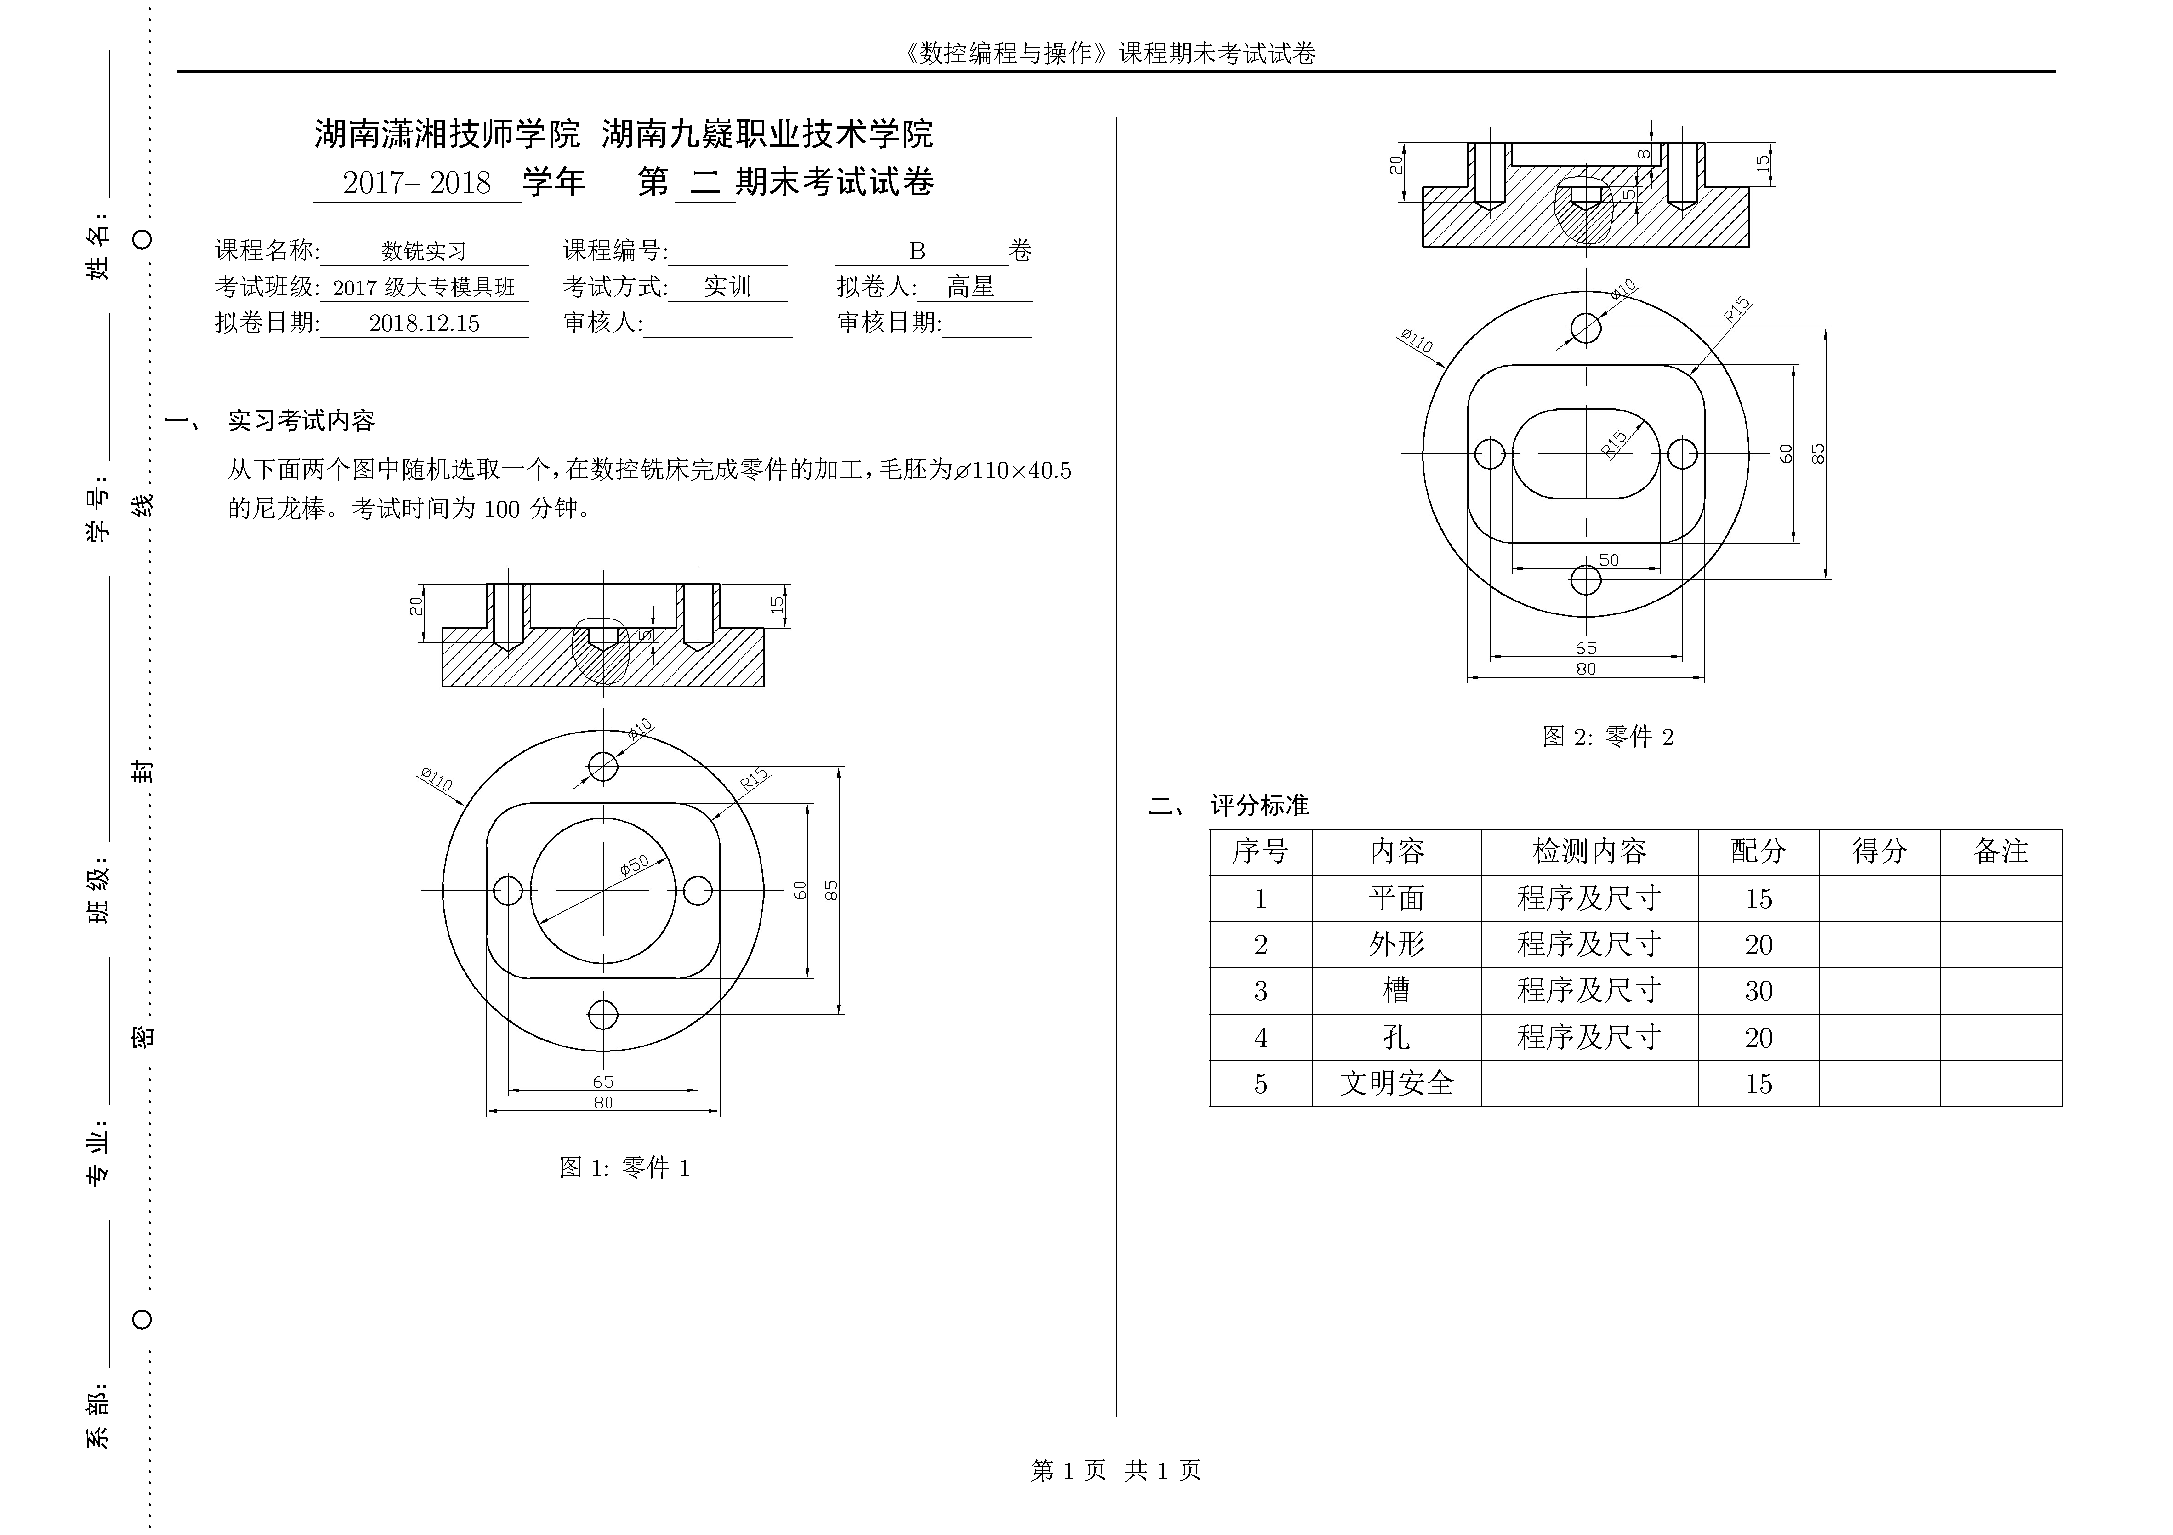
\includepdf[pages={-},landscape=true]{shijuan.pdf}
%
%\newpage
%\addcontentsline{toc}{section}{期末试卷答案}
%\includepdf[pages={-},landscape=true]{shijuan-daan.pdf}
%
%\newpage
%\addcontentsline{toc}{section}{学生成绩}
%\includepdf[pages={-},landscape=true]{chenzhi.pdf}
%
%\newpage
%\addcontentsline{toc}{section}{试卷分析}
%\include{data/shijuanfenxi}
%
%\newpage
%\addcontentsline{toc}{section}{教学总结}
%\renewcommand{\baselinestretch}{1.3}
%{
%\begin{center}
%	\huge \heiti 教 ~ 学  ~总  ~结
%\end{center}
%
% \large  \setlength{\parindent}{2em} 
% 
%《加工中心编程、仿真与操作》是15级中数班的一门专业课,
% 本课程已在上一学期中,就学习了手工编程的基本知识。
% 本学期主要学习简化编程与宏程序,及常见零件的加工工艺。
% 通过本学期的教学,完成了教学任务,基本达到教学目标,教学效果较好。
%
%本学期实习课共分4个课题,都在计划的时间内完成课题的实施,
%有少同学没有完成课题。通过期末考试,大部分的同学掌握的比较好,
%也就是2/3的同学掌握了所学的知识。实习大部分同学完成了课题,
%达到教学目标,教学效果较好。
%
%本学的仿真课主要学习《MasterCAM》自动编程,
%包括二维绘图,二维加工,三维空间曲线,三维曲面及实体,三维加工,
%以及每个课题的仿真模拟等。完成的全部教学。
%
%本学期在教学过程中主要的所用的教学方法为分析引导,
%通过实例进行讲解,仿真与实习相互融通。在进行宏程序入门教学过程中,
%进行实例设计,引导学生进行学习,效果好,工艺课在教学中要多讨论,
%实习课中要引导学生进行自我总结。
%
%在教学中有部分学生厌学,旷课需要进行一步的提高学生们的兴趣,
%在仿真课上,学生们的自觉性较差时,最好安排课题让学生们做。
%要进一步的加强教学管理,并及时与班主任进行联系,沟通。
%以便取得更好的教学效果。

%\newpage
%\addcontentsline{toc}{section}{封面-后}
%\pagestyle{empty}
%\begin{center}
%	\huge \heiti 教 ~~学 ~~检 ~~查 ~~记~~ 录
%	
%	\songti\normalsize 
%	\begin{tabu} to \textwidth {|X[1,c,m]|X[10,r,m]|N}
%		\hline
%	\multirow{1}{1em}{\large 系部意见}  &\vspace{7cm}  检查人签名(盖章) 
%	\hspace{4cm} \par  二〇 \underline{\hspace{2em}}   
%	年\underline{\hspace{1em}}   月 \underline{\hspace{1em}}  日 
%	\hspace{1cm}  \par &\\ [7.5cm] \hline
%	\multirow{1}{1em}{\large 教务处意见} & \vspace{7cm}  检查人签名(盖章) 
%	\hspace{4cm} \par  二 〇  \underline{\hspace{2em}} 年  
%	\underline{\hspace{1em}} 月 \underline{\hspace{1em}}  日 \hspace{1cm} 
%	\par & \\[7.cm] \hline	
%	\end{tabu}
%\end{center}




%中文习惯是设定首行缩进为2em。注意此设置一定要在document环境之中,这可能与setlength 作用范围相关
%\setlength{\parindent}{2em}                    
%
%\title{Xecjk Template Test}
%\author{Xiao Hanyu}
%\maketitle
%
%\tableofcontents
%\listoffigures
%%\listoftablescontent
%
%\include{data/content}
%\include{data/appendix}
%
%%% 加入参考文献支持
%\bibliography{data/main}
%%% 解决目录中没有相应的参考文献的条目问题
%\addcontentsline{toc}{section}{\refname} 
\end{document}
%%%% 正文部分结束
%%%%%%%%------------------------------------------------------------------------
